\documentclass[conference]{IEEEtran}
\IEEEoverridecommandlockouts
% The preceding line is only needed to identify funding in the first footnote. If that is unneeded, please comment it out.
%Template version as of 6/27/2024

\usepackage{cite}
\usepackage{amsmath,amssymb,amsfonts}
\usepackage{algorithmic}
\usepackage{graphicx}
\usepackage{textcomp}
\usepackage{xcolor}
\def\BibTeX{{\rm B\kern-.05em{\sc i\kern-.025em b}\kern-.08em
T\kern-.1667em\lower.7ex\hbox{E}\kern-.125emX}}
\begin{document}

\title{Conference Paper Title*\\
    \thanks{Identify applicable funding agency here. If none, delete this.}
}

\author{\IEEEauthorblockN{1\textsuperscript{st} Brenda Silva de Alencar}
    \IEEEauthorblockA{\textit{Universidade Federal da Bahia (UFBA)} \\
        Salvador, Brasil \\
        brenda.s1602@outlook.com}
}

\maketitle

\begin{abstract}
    This document is a model and instructions for \LaTeX.
    This and the IEEEtran.cls file define the components of your paper [title,
            text, heads, etc.]. *CRITICAL: Do Not Use Symbols, Special
    Characters,
    Footnotes,
    or Math in Paper Title or Abstract.
\end{abstract}

\begin{IEEEkeywords}
    component, formatting, style, styling, insert.
\end{IEEEkeywords}

\section{Introduction}
A utilização de energia solar no Brasil tem crescido nos últimos anos. De
acordo com [X] o uso de
placas solares está em XX. A eficiência de sistemas de energia solar é
comumente afetada pela presença de
defeitos nas células fotovoltaicas, como fissuras, áreas inativas,
e \textit{gridlines}. Sendo assim, a inspeção dos módulos é imprescindível para
obter-se um maior aproveitamento dos ativos.

    [Matos] aponta o ensaio de eletroluminescência
em módulos fotovoltaicos como uma ferramenta recorrente na detecção de
defeitos. Durante o ensaio, o módulo examinado é colocado em ambiente escuro e
submetido à uma corrente elétrica direta, com valor semelhante à sua corrente
de curto circuito nominal.  Em seguida, capturam-se imagens do módulo
utilizando uma câmera com sensor de infravermelho capaz de capturar a radiação,
normalmente na faixa de 800
a 1150 nm, emitida pelas células (Frazão et al.,2016). Este método
não-destrutivo é eficaz em detectar anomalias que não são
reveladas na
inspeção visual. Entretanto, neste processo, é necessário que centenas de
imagens sejam revisadas por um técnico, o que compromete
significativamente a eficiência da inspeção de um grande volume de módulos,
como em plantas de energia
solar e em linhas de produção em fábricas de módulos fotovoltaicos.

Desde a expansão das técnicas de aprendizado de máquina, o uso dessas
tecnologias têm se tornado cada vez mais comum na detecção de defeitos em
células fotovoltaicas.A grande quantidade de dados gerados em um ensaio de
eletroluminescência pode ser processada por algoritmos de aprendizado de
máquina, que são capazes de identificar padrões em imagens e classificar as
células fotovoltaicas como defeituosas ou não. [Deitsch] propôs dois modelos
para determinar a probabilidade de uma célula estar danificada, o primeiro
utiliza a arquitetura
Máquina de Vetores de Suporte (SVM) e o segundo usa uma Rede Neural
Convolucional (CNN). O primeiro modelo atingiu uma acurácia média de 82.44\%,
enquanto o segundo atingiu 88.42\%. Em trabalhos mais recentes ([],[]), são
utilizados modelos de segmentação de imagem baseados em aprendizagem profundo
de máquina para classificar defeitos e características encontradas das células
fotovoltaicas. [] avaliou a eficácia de x modelos treinados para classificar
24 tipos de defeitos e características em células fotovoltaicas.
Dentre os modelos analisados, o DeepLabv3+ e o U-Net obtiveram os melhores
resultados, obtendo um recall de 86\% e XXX na identificação de fissuras.

Este trabalho apresenta um modelo baseado em aprendizagem de máquina para
detecção de células fotovoltaicas defeituosas. O modelo proposto determina a
possibilidade da célula estar danificada utilizando uma arquitetura de rede
neural convolucional (CNN). O treinamento foi realizado com imagens de
eletroluminescência de células fotovoltaicas disponibilizadas por [X].

\section{Desenvolvimento}

Fig.\ref{fig:metodologia} sintetiza a metodologia nas etapas
"pré-processamento", metodologia
"treinamento" e "predição", discutidas nas sessões a seguir.
\begin{figure}[htbp]
    \centerline{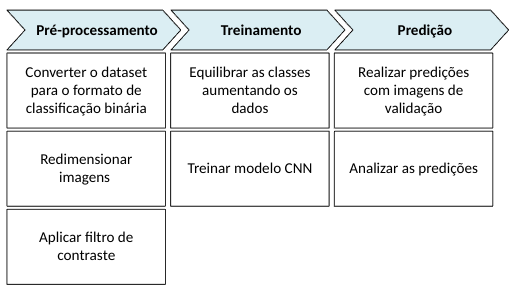
\includegraphics[width=0.5\textwidth]{images/metodologia.png}}
    \caption{Example of a figure caption.}
    \label{fig:metodologia}
\end{figure}

\subsection{Pré-processamento}\label{AA}

O conjunto de dados utilizado para este trabalho é fornecido por [x]. Este
dataset contêm 2.426 imagens de eletroluminescência de células de painéis
solares reais. Cada imagem no dataset contém uma célula individual de silício
policristalino ou monocristalino. Todas as imagens foram rotuladas por um
especialista,
indicando a probabilidade da célula estar danificada.

Durante a etapa de pré-processamento, os valores de
probabilidade são convertidos em uma classe binária, classificando as imagens
como "Defeituosa" ou "Não Defeituosa". Nesse processo imagens rotuladas com
probabilidade acima de 60\% são categorizadas como "Defeituosa", enquanto
aquelas com uma probabilidade igual ou inferior a este limiar são rotuladas
como "Não Defeituosa". Em seguida, as imagens foram redimensionadas para
224x224 pixels. Na Fig.\ref{fig:amostras-dataset} são apresentadas quatro
amostras do
dataset reclassificado.

\begin{figure}[htbp]
    \centering
    \begin{tabular}{cc}
        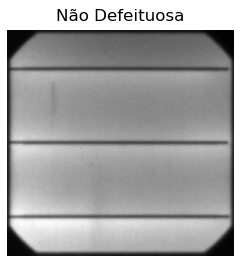
\includegraphics[width=0.20\textwidth]{images/mono-no-defect.png} &
        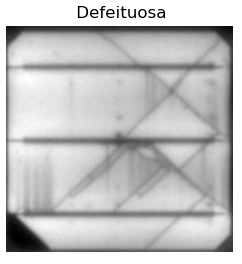
\includegraphics[width=0.20\textwidth]{images/mono-defect.png}
        \\
        \textbf{2 (a)}                                                    &
        \textbf{2 (b)}                                                      \\
        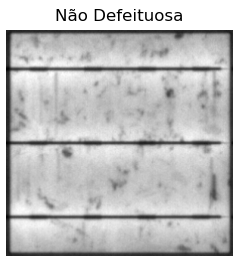
\includegraphics[width=0.20\textwidth]{images/poly-no-defect.png} &
        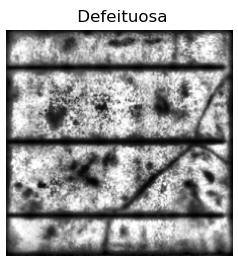
\includegraphics[width=0.20\textwidth]{images/poly-defect.png}
        \\
        \textbf{2 (c)}                                                    &
        \textbf{2 (d)}                                                      \\
    \end{tabular}
    \caption{Amostras do dataset de células fotovoltaicas: 2(a) monocristalina
        sem defeito, 2(b) monocristalina com defeito, 2(c) policristalina sem
        defeito,
        2(d) policristalina com defeito. [REFER]}
    \label{fig:amostras-dataset}
\end{figure}

Mesmo após este processo, a disposição das classes no dataset
estava desbalanceada, pois as células com defeitos representavam apenas
31.3\% do total de imagens. Para contornar este problema, foi empregado
o método de aumento de dados no conjunto de imagens classificadas como
"Defeituosa", com o auxílio da biblioteca XXX. O gráfico na
Fig.\ref{fig:metodologia} apresenta a disposição final do dataset de
referência.

\subsection{Treinamento}\label{AA}

O dataset processado foi dividido de forma randômica em dois conjuntos, um de
treinamento
com 75\% (XX imagens) e outro de teste com 24\% (XX imagens). Os
hiperparâmetros do modelo foram definidos empiricamente, com base em
experimentos com um dataset
reduzido e ajustes realizados durante o processo de desenvolvimento. Então o
modelo proposto,
uma rede convolucional, foi treinado a classificar uma célula fotovoltaica como
"Defeituosa" ou "Não
Defeituosa".

\begin{table}[htbp]
    \caption{Table Type Styles}
    \begin{center}
        \begin{tabular}{|c|c|c|c|}
            \hline
            \textbf{Table}            & \multicolumn{3}{|c|}{\textbf{Table
                    Column Head}}
            \\
            \cline{2-4}
            \textbf{Head}             & \textbf{\textit{Table column subhead}}
                                      &
            \textbf{\textit{Subhead}} & \textbf{\textit{Subhead}}
            \\
            \hline
            copy                      & More table copy$^{\mathrm{a}}$
                                      &
                                      &
            \\
            \hline
            \multicolumn{4}{l}{$^{\mathrm{a}}$Sample of a Table footnote.}
        \end{tabular}
        \label{tab1}
    \end{center}
\end{table}
\subsection{Predição}\label{AA}

Na última etapa, foram realizadas predições com o modelo treinado utilizando
um conjunto de 15 imagens. Além disso, avaliou-se a eficácia do modelo proposto
por meio de métricas de avaliação, como acurácia, precisão, recall e F1-score.

\section{Resultados}

A acurácia do modelo proposto foi de XX\%, com uma precisão de XX\%, recall de
XX\%. Fig \ref{fig:confusion-matrix} apresenta a matriz de confusão do modelo,
enfatizando que
o modelo obteve um bom desempenho na classificação de células fotovoltaicas
....,

\section{Conclusão}

\section*{Acknowledgment}

The preferred spelling of the word ``acknowledgment'' in America is without
an ``e'' after the ``g''. Avoid the stilted expression ``one of us (R. B.
G.) thanks $\ldots$''. Instead, try ``R. B. G. thanks$\ldots$''. Put sponsor
acknowledgments in the unnumbered footnote on the first page.

\section*{References}

Please number citations consecutively within brackets \cite{b1}. The
sentence punctuation follows the bracket \cite{b2}. Refer simply to the
reference
number, as in \cite{b3}---do not use ``Ref. \cite{b3}'' or ``reference
\cite{b3}'' except at
the beginning of a sentence: ``Reference \cite{b3} was the first $\ldots$''

Number footnotes separately in superscripts. Place the actual footnote at
the bottom of the column in which it was cited. Do not put footnotes in the
abstract or reference list. Use letters for table footnotes.

Unless there are six authors or more give all authors' names; do not use
``et al.''. Papers that have not been published, even if they have been
submitted for publication, should be cited as ``unpublished'' \cite{b4}. Papers

that have been accepted for publication should be cited as ``in press''
\cite{b5}.
Capitalize only the first word in a paper title, except for proper nouns and
element symbols.

For papers published in translation journals, please give the English
citation first, followed by the original foreign-language citation \cite{b6}.

\begin{thebibliography}{00}
    \bibitem{b1} G. Eason, B. Noble, and I. N. Sneddon, ``On certain integrals
    of
    Lipschitz-Hankel type involving products of Bessel functions,'' Phil.
    Trans.
    Roy. Soc. London, vol. A247, pp. 529--551, April 1955.
    \bibitem{b2} J. Clerk Maxwell, A Treatise on Electricity and Magnetism, 3rd
    ed., vol. 2. Oxford: Clarendon, 1892, pp.68--73.
    \bibitem{b3} I. S. Jacobs and C. P. Bean, ``Fine particles, thin films and
    exchange anisotropy,'' in Magnetism, vol. III, G. T. Rado and H. Suhl, Eds.
    New
    York: Academic, 1963, pp. 271--350.
    \bibitem{b4} K. Elissa, ``Title of paper if known,'' unpublished.
    \bibitem{b5} R. Nicole, ``Title of paper with only first word
    capitalized,'' J.
    Name Stand. Abbrev., in press.
    \bibitem{b6} Y. Yorozu, M. Hirano, K. Oka, and Y. Tagawa, ``Electron
    spectroscopy studies on magneto-optical media and plastic substrate
    interface,'' IEEE Transl. J. Magn. Japan, vol. 2, pp. 740--741, August 1987
        [Digests 9th Annual Conf. Magnetics Japan, p. 301, 1982].
    \bibitem{b7} M. Young, The Technical Writer's Handbook. Mill Valley, CA:
    University Science, 1989.
    \bibitem{b8} D. P. Kingma and M. Welling, ``Auto-encoding variational
    Bayes,''
    2013, arXiv:1312.6114. [Online]. Available: https://arxiv.org/abs/1312.6114
    \bibitem{b9} S. Liu, ``Wi-Fi Energy Detection Testbed (12MTC),'' 2023,
    gitHub
    repository. [Online]. Available:
    https://github.com/liustone99/Wi-Fi-Energy-Detection-Testbed-12MTC
    \bibitem{b10} ``Treatment episode data set: discharges (TEDS-D):
    concatenated,
    2006 to 2009.'' U.S. Department of Health and Human Services, Substance
    Abuse
    and Mental Health Services Administration, Office of Applied Studies,
    August,
    2013, DOI:10.3886/ICPSR30122.v2
    \bibitem{b11} K. Eves and J. Valasek, ``Adaptive control for singularly
    perturbed systems examples,'' Code Ocean, Aug. 2023. [Online]. Available:
    https://codeocean.com/capsule/4989235/tree

    @article{PRATT2023200048,
        title = {A benchmark dataset for defect detection and classification in
                electroluminescence images of PV modules using semantic
                segmentation},
        journal = {Systems and Soft Computing},
        volume = {5},
        pages = {200048},
        year = {2023},
        issn = {2772-9419},
        doi = {https://doi.org/10.1016/j.sasc.2023.200048},
        url =

            {https://www.sciencedirect.com/science/article/pii/S2772941923000017},
        author = {Lawrence Pratt and Jana Mattheus and Richard Klein},
        keywords = {Electroluminescence, EL, PV, Semantic segmentation, Machine
                learning}
    }

\end{thebibliography}

\vspace{12pt}
\color{red}
IEEE conference templates contain guidance text for composing and formatting
conference papers. Please ensure that all template text is removed from your
conference paper prior to submission to the conference. Failure to remove the
template text from your paper may result in your paper not being published.

\end{document}
